\chapter[Simple SLAM]{Simple SLAM: Auto-localização Simplificada}

Neste capítulo, são apresentados todos os componentes presentes no \textit{Simple SLAM}, incluindo a etapa de montagem do robô,
a configuração do ambiente de programação e do ambiente de navegação do robô, buscando padronizar ao máximo as características da
pesquisa para que a mesma possa ser aplicada e analisada por outro pesquisador.

\section{Contextualização}
\label{sec:simple_context}

	O principal incentivo do pesquisador em relação a esta proposta de trabalho faz referência às metodologias de ensino de matemática, física e programação, tanto no âmbito da graduação, quanto nos ensinos Básico, Fundamental e Médio. Assim como já foi apresentado durante o trabalho, mais especificamente na seção \ref{sec:robótica_educacional}, as metodologias de ensino geralmente aplicadas nos Centros Educacionais possuem uma característica de ensino passiva e ultrapassada. Desse modo, buscando garantir maior interesse dos alunos nos conteúdos apresentados, a Robótica Educacional é vista como uma ferramenta eficiente de ensino, como apresentam \cite{teachingWithRoboticKit}, \cite{construcionismoPapert} e \cite{roboticaEducativaEnsinoMedio}.

	Com isto em mente, o \textit{Simple SLAM} busca apresentar diversas técnicas de auto-localização que podem ser utilizadas como uma atividade Educacional, em um contexto de ensino. Além disso, o \textit{Simple SLAM} tem como objetivo a implementação de técnicas de auto-localização utilizadas no alto nível da robótica mundial em um contexto simplificado,
	ou seja, em um cenário tipicamente associado à Robótica Educacional. Nesse cenário, estão presentes a falta de recursos, o uso de kits mais
	padronizados e até mesmo limitados em termos de recursos e/ou de sensores e atuadores. No caso desse trabalho, foram utilizados
	equipamentos e recursos disponíveis no kit de Robótica da LEGO - NXT.

  Em relação as técnicas de alto nível da Robótica Móvel, esta pesquisa busca implementar e analisar a técnica de Localização a partir da utilização
	do Filtro de Partículas, ou Filtro de Monte Carlo. Como foi apresentado na seção \ref{sub:filtro_de_partículas}, o mesmo envolve
	a manipulação de técnicas probabilísticas com o intuito de obter a localização atual do robô.

	Durante a primeira etapa desta pesquisa, foram analisadas algumas das técnicas mais utilizadas no contexto mundial da robótica móvel, como o Filtro de Kalman e
	o Filtro de Partículas. Estas duas técnicas possuem como objetivo possibilitar a análise da posição atual do robô a partir do uso da probabilidade. Durante a realização
	da Revisão Sistemática, documentada na seção \ref{sec:revisão_sistemática}, foi observado que a técnica do Filtro de Kalman se encontra
	como a técnica probabilística mais utilizada no contexto mundial da robótica móvel, estudada e difundida desde a década de 60, com exemplos de aplicações
	nos mais diversos contextos, geralmente ligados a sistemas de controle.

	Já o Filtro de Partículas, de acordo com \cite{sequestro}, é uma técnica que, apesar de ter surgido há muitos anos, com
	pesquisas relacionadas à mesma durante a Segunda Guerra Mundial, só vem se tornando um foco maior de pesquisas e análises relacionadas
	a Robótica Móvel ao longo da última década. Desse modo, como o intuito deste trabalho é pesquisar e analisar a utilização de técnicas de auto-localização em um contexto
	limitado da robótica movel, optou-se pela utilização da técnica do Filtro de Partículas, uma técnica consideravelmente nova no contexto da
	robótica mundial.

	Além da importância da realização de pesquisas relacionadas a técnicas que vêm buscando espaço na comunidade de robótica, a escolha da técnica dá-se, ainda,
	pela possibilidade de resolução do problema do \textit{sequestro do robô}, apresentado por \cite{sequestro}, o qual pode ser solucionado ao se utilizar a técnica do
	Filtro de Partículas, diferentemente da utilização do Filtro de Kalman, como foi descrito na seção \ref{sub:filtro_de_partículas}.

\section{Arquitetura do Robô}

De acordo com \cite{vieira}, a arquitetura de robôs móveis pode ser sub-dividida em cinco camadas: \textit{percepção}, \textit{decisão}, \textit{planejamento de caminho}, \textit{geração de trajetória} e \textit{sistema de controle}.

A primeira camada, denominada \textit{camada de percepção}, foi o grande foco deste trabalho, onde a identificação de obstáculos como pontos de referência é uma atividade essencial para a possibilidade de auto-localização, utilizando como base o Filtro de Partículas, por exemplo. Esta camada é responsável por adquirir informações sobre o ambiente ao seu redor, viabilizando a navegação e auto-localização no mesmo.

Já a segunda camada, \textit{decisão}, que foi o foco de trabalho de \cite{tccCarol}, tem como responsabilidade processar decisões do
robô. Nesta camada, se encontra o verdadeiro cérebro do robo, como afirma \cite{vieira}.

Na terceira camada, \textit{planejamento de caminho}, será utilizado, como ferramenta de apoio, o \textit{framework} Traveller, desenvolvido por \cite{tccRodrigo}. Sua utilização se refere ao planejamento da navegação no ambiente após o mapeamento, mesmo que parcial, do ambiente. Ou seja, enquanto o robô navega e mapeia o ambiente, os locais já percorridos (conhecidos e mapeados) possibilitarão a utilização do \textit{framework}. Por outro lado, em locais ainda desconhecidos, o planejamento do caminho será feito de forma aleatória, buscando mapear o ambiente como um todo.

A quarta camada, \textit{geração da trajetória}, utiliza o planejamento realizado na camada anterior para definir quais açoes devem ser realizadas no \textit{hardware} do robô, levando em consideração as características físicas do mesmo. Com isso, a quinta camada, \textit{sistema de controle}, é chamada para verificar o recebimento adequado dos sinais, assim como sua execução nos atuadores.

A Figura \ref{img:camadas} apresenta as cinco camadas, nas quais, em seu nível mais alto, encontra-se a camada de percepção, que é o foco deste trabalho.

\begin{figure}[H]
	\centering
	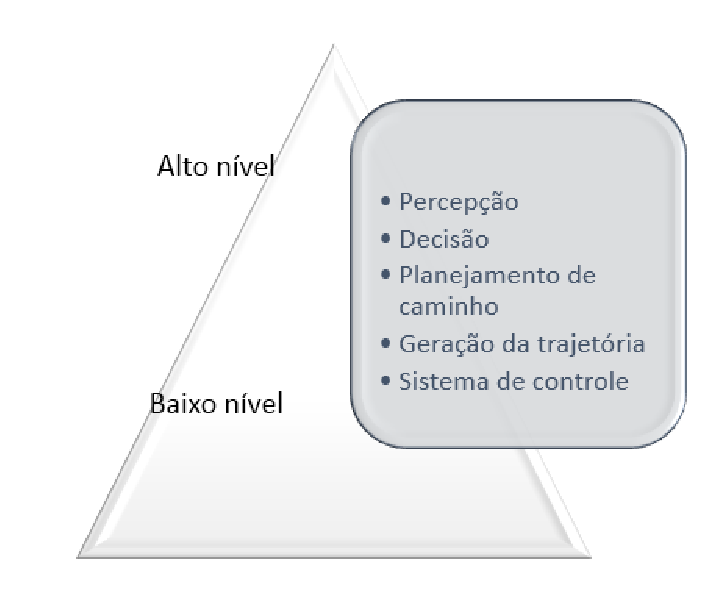
\includegraphics[scale=0.6]{figuras/camadas.eps}
	\caption[Arquitetura do Robô]{Arquitetura do Robô. Fonte \cite{vieira}.}
	\label{img:camadas}
\end{figure}

\section{Montagem do Robô}
\label{sec:montagem_robo}

	Esta seção tem como objetivo apresentar a forma de montagem do robô utilizada durante a pesquisa. O padrão utilizado foi escolhido após a análise e comparação da margem de erro presente em dois tipos de montagem. Durante a primeira etapa deste trabalho (TCC 1), foi utilizado o robô montado com esteiras para movimentação, seguindo o padrão encontrado em tanques de guerra, como pode ser observado na Figura \ref{img:montagem_antiga}.

	{\centering
	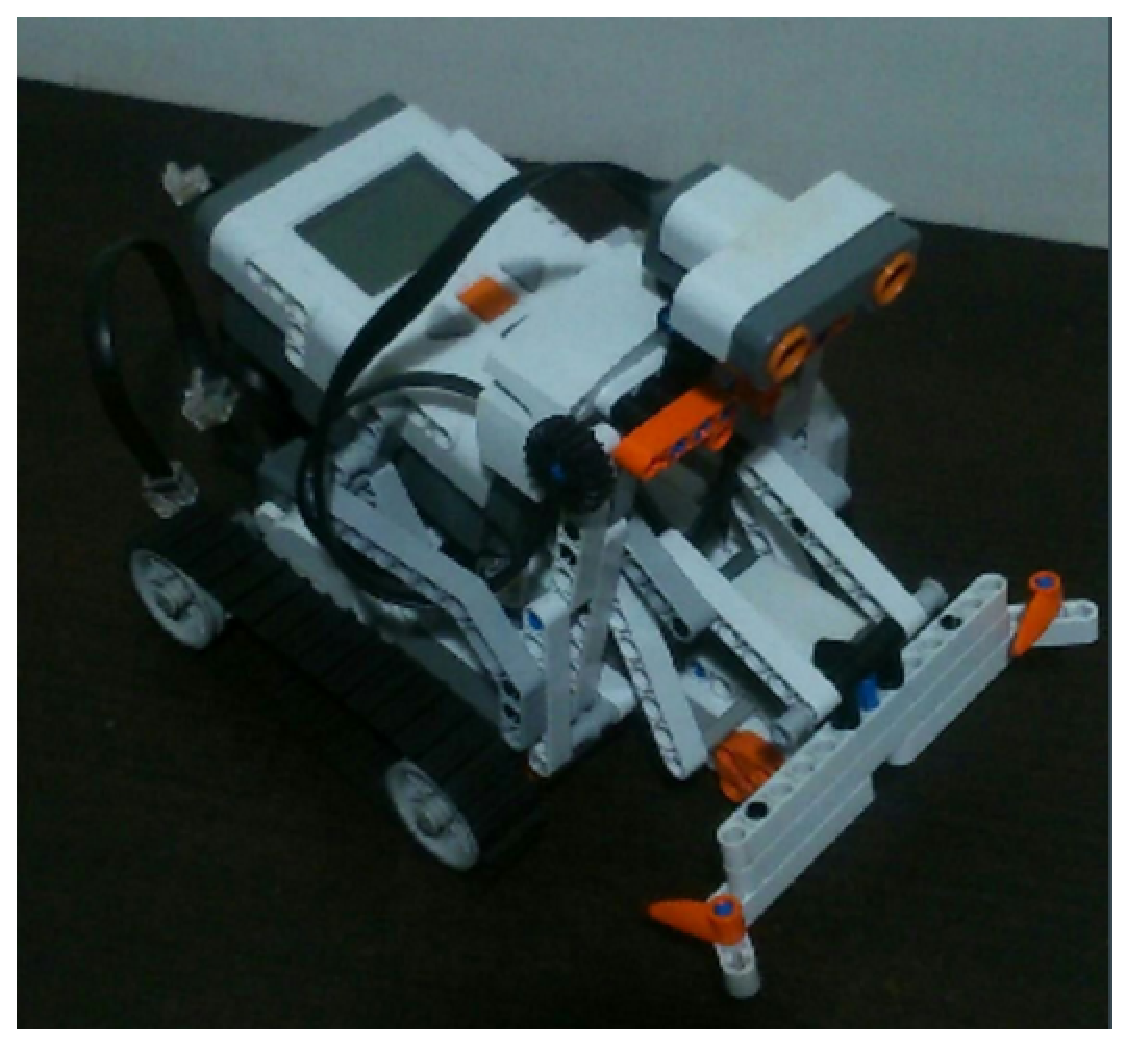
\includegraphics[scale=0.4]{figuras/montagem_antiga.eps}
	\captionof{figure}{Montagem do Robô Durante o TCC 1}
	\label{img:montagem_antiga}
	\par}

	Entretanto, após algumas análises e pesquisas, concluiu-se que a utilização de esteiras maximiza a margem de erro durante a navegação, prejudicando a qualidade do movimento. Isto se dá, segundo \cite{legonxj}, devido a área de contato entre a esteira e o chão. Quanto maior a área de contato, mais crítico é o resultado de derrapagens durante a movimentação, inviabilizando sua utilização para este objetivo. Desse modo, a partir da segunda etapa desta pesquisa, passou-se a utilizar um robô do tipo \textit{Carpet} (de acordo com a nomenclatura da LEGO), no qual estão presentes duas rodas motorizadas e uma terceira roda para equilíbrio do robô.

	Além do padrão relacionado às rodas, deve-se atentar a localização do sensor de distância. Este deve estar localizado exatamente no centro do robô, ou o mais próximo desse ponto. As Figuras \ref{img:montagem_robo}  e \ref{img:montagem_robo_costas} apresentam o robô utilizado durante a segunda etapa desta pesquisa.

	{\centering
	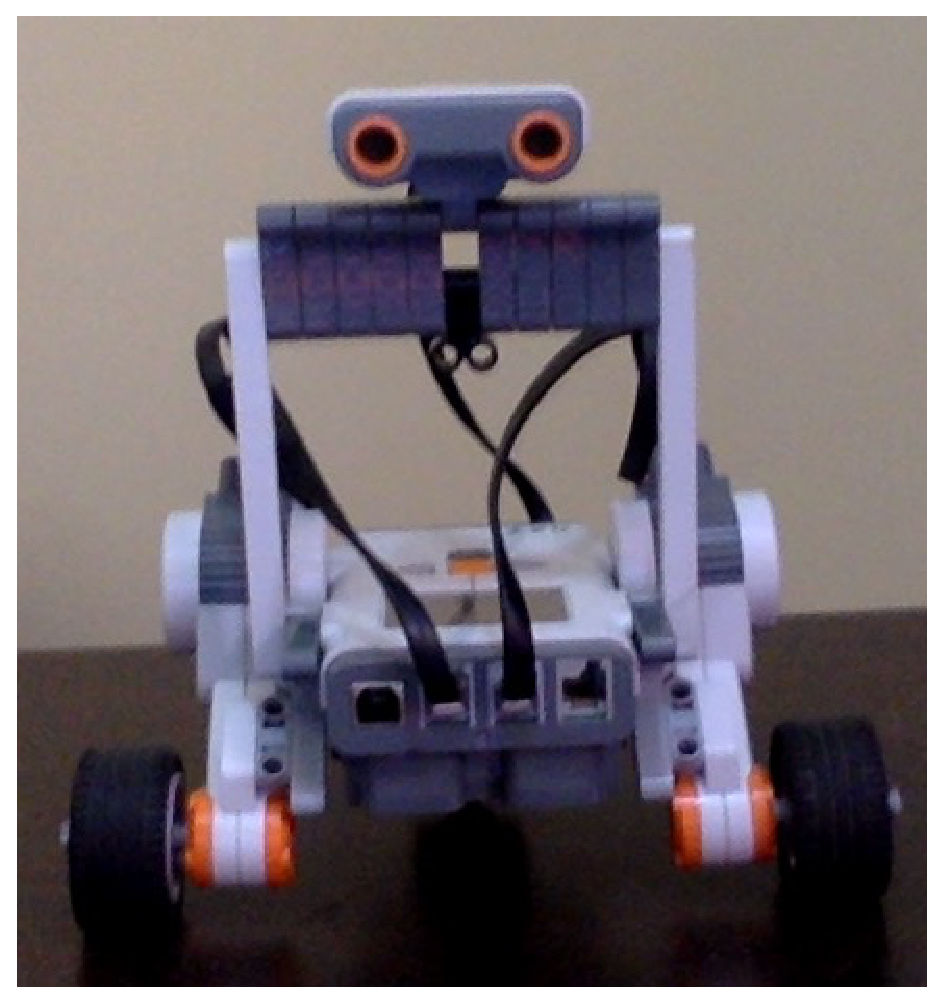
\includegraphics[scale=0.5]{figuras/frente.eps}
	\captionof{figure}{Montagem do Robô Durante o TCC 2 - Frente}
	\label{img:montagem_robo}
	\par}

	A terceira roda, utilizada apenas como roda de apoio, é feita a partir de uma simples montagem de peças LEGO, como pode ser observado na Figura \ref{img:montagem_robo_costas}.

	{\centering
	\includegraphics[scale=0.25]{figuras/rodinha.eps}
	\captionof{figure}{Montagem do Robô Durante o TCC 2 - Roda de Apoio}
	\label{img:montagem_robo_costas}
	\par}

	Em relação ao código utilizado durante a pesquisa, as portas utilizadas para acesso aos motores e sensores seguem o padrão apresentado na Tabela \ref{tab:portas_motores_sensores}.

	\begin{table}[H]
		\centering
		\caption{Configuração dos Componentes Utilizados}
		\label{tab:portas_motores_sensores}
		\begin{tabular}{|c|c|}
		\hline
		\textbf{Porta} & \textbf{Componente} \\ \hline
		B              & Motor esquerdo      \\ \hline
		C              & Motor direito       \\ \hline
		S1             & Sonar               \\ \hline
		\end{tabular}
	\end{table}

\section{Ambiente de Navegação}

	Esta seção tem como objetivo apresentar o ambiente de navegação utilizado durante a realização da pesquisa. Ao longo da mesma, diversos ambientes foram utilizados, possibilitando a escolha da melhor configuração para análise efetiva dos resultados.

	Sabe-se que, independente do piso selecionado, erros estarão presentes, seja devido a deslizes entre as rodas e o piso, ou devido a margem de erro presente nos sensores odométricos. Desse modo, buscou-se selecionar um piso que possibilite uma margem de erro mínima, dentre as opções presentes em um contexto simplificado, de uma escola, por exemplo.

	Deve-se optar sempre por pisos lisos, ou seja, sem irregularidades, as quais podem `travar' a roda de apoio, que não possui um formato tão adequado quanto as rodas motorizadas. De acordo com análises empíricas durante a realização da pesqisa,
	identificou-se que este formato diferenciado da roda de apoio, o qual pode ser visualizado na Figura \ref{img:montagem_robo_costas}, pode gerar diversas interferências durante a navegação, principalmente em pisos que possuem `rachaduras', como as presentes em pisos feitos com azulejo, por exemplo.

	Devido a esta característica da roda de apoio, pisos feitos com azulejo devem ser evitados, optando sempre por pisos tão lisos quanto possível. Um exemplo do piso utilizado durante esta pesquisa pode ser visualizado na Figura \ref{img:piso_ambiente}.

	{\centering
	\includegraphics[scale=0.2]{figuras/real_cen1_ex1.eps}
	\captionof{figure}{Exemplo de Piso.}
	\label{img:piso_ambiente}
	\par}

	Com o piso definido, deve-se definir o padrão de obstáculos no ambiente. Como o objetivo desta pesquisa é analisar a viabilidade da utilização de técnicas de auto-localização e mapeamento de ambientes em robôs simples, utilizando apenas um sensor de distância do tipo \textit{sonar}, deve-se adequar o padrão de obstáculos no ambiente, buscando minimizar a margem de erro presente na análise.

	Para que o robô seja capaz de se localizar no ambiente, o mesmo precisa identificar características únicas no mesmo. Isto é feito utilizando
	os obstáculos presentes no ambiente. Desse modo, a presença de obstáculos no mapa é essencial para a viabilidade do processo de
	auto-localização. Para que a identificação dos obstáculos como \textit{pontos de referência} seja possível, os mesmos precisam
	se adequar ao máximo às características presentes nos sonares. A principal característica do sonar utilizado é apresentada na
	Figura \ref{img:cone}, a qual envolve o modelo de emissão do sinal utilizado pelo sonar, em formato de cone.

	Para que um sonar funcione, o mesmo emite um sinal que irá refletir no primeiro obstáculo encontrado, retornando ao robô e, a partir da análise do tempo gasto para percorrer este caminho, chega-se a conclusão da distância entre o robô e o objeto que refletiu o sinal. Porém, este sinal não é emitido de forma unidimensional, sua emissão é feita no formato de cone, devido as características físicas relacionadas à tramissão do som no ar. Por esse motivo, alguns erros podem ser adicionados à solução, visto que em determinadas situações, o objeto que refletiu o sinal sonoro não se encontra exatamente à frente do robô.

	Isto significa que o robô pode enxergar obstáculos mesmo quando não existe nenhum obstáculo diretamente à sua frente, enxergando obstáculos presentes nas laterais e tratando-os como obstáculos frontais.
	Infelizmente, não foi possível encontrar uma solução exata para esse problema. Isso se deve ao fato de usar um sonar para detecção de distâncias, com o qual é intrínseco esse tipo de problema.
	Desse modo, buscando minimizar a taxa de ocorrência desse \textit{'engano'}, o ambiente foi pensado e criado utilizando paredes lisas e em formatos uniformes, retilíneos.

	Como o objetivo da pesquisa é analisar a possibilidade da auto-localização dentro de um ambiente, optou-se pela não utilização de obstáculos entre as paredes. Fazendo com que o ambiente seja composto apenas de piso e paredes, como apresenta a Figura \ref{img:exemplo_ambiente}.

	Como o robô deverá analisar os pontos de referência (paredes), a partir de determinadas características, e se auto-localizar em
	relação ao mapa, o ambiente utilizado não pode ser simétrico. Dessa forma, deve-se evitar a utilização de ambientes quadrados ou retangulares, por exemplo, já que o robô não conseguiria identificar características únicas em cada local do ambiente.
	A Figura \ref{img:exemplo_ambiente} apresenta uma boa opção de ambiente a ser utilizado, já que o mesmo possui características que viabilizam a comparação e conclusão de unicidade.

	\begin{figure}[H]
		\centering
		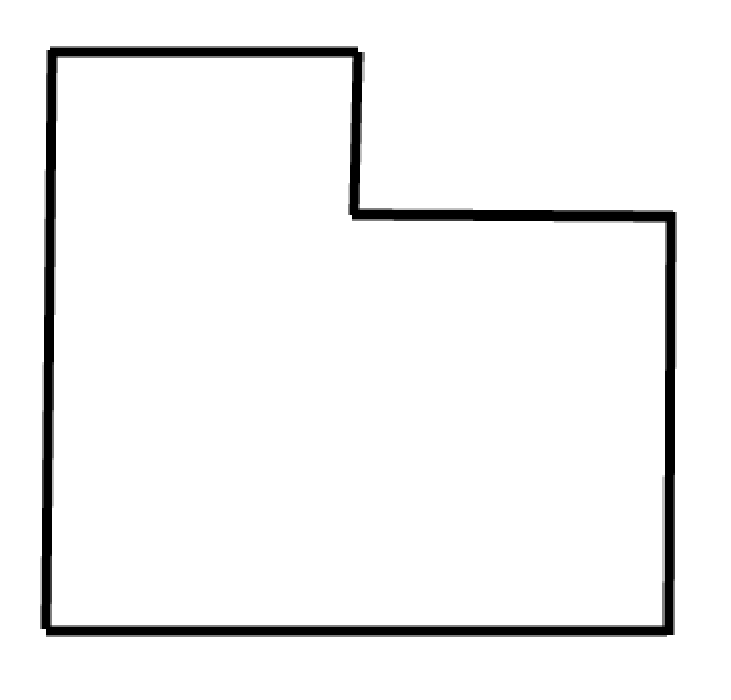
\includegraphics[scale=0.5]{figuras/exemplo_ambiente.eps}
		\caption[Exemplo de Ambiente]{Exemplo de Ambiente.}
		\label{img:exemplo_ambiente}
	\end{figure}

\section{Configuração e Integração das Tecnologias}

Nesta seção, será apresentado o passo a passo para configuração e integração das tecnologias utilizadas durante este trabalho. A principal tecnologia utilizada é o pacote leJOS (Lego Java Operating System) NXJ, o qual possibilita a utilização da linguagem Java para implementação dos algoritmos durante a realização do trabalho.
A tecnologia leJOS NXJ envolve um ambiente Java, um \textit{firmware} e uma API, como descrito na seção \ref{sub:lejos_nxj}.

O ambiente java disponibilizado pelo leJOS NXJ possibilita integração com a IDE Eclipse, facilitando o \textit{upload} de códigos, atualização de \textit{firmware} e utilização da API. O \textit{firmware} é necessário, pois cria uma máquina virtual Java no NXT, possibilitando a execução de códigos Java no \textit{Brick}.
Além disso, a API leJOS envolve uma variedade de classes e métodos com algoritmos já produzidos e disponibilizados para utilização durante o desenvolvimento. Com a utilização da API, o desenvolvedor não se preocupa com a implementação de algoritmos comuns, como de navegação e obtenção de dados dos sensores.

A plataforma leJOS NXJ é multiplataforma, possibilitando sua utilização no \textit{Windows}, \textit{Linux} e \textit{MAC OS}. Nas seções a seguir apresentadas, são descritos os passos para instalação e configuração do leJOS NXJ nas três plataformas.

\subsection{Instalação no Windows} % (fold)
\label{sub:instalação_no_windows}

	Primeiramente, para possibilitar a comunicação entre o PC e o NXT, deve-se instalar um \textit{USB Driver}, o qual pode ser encontrado \href{https://www.lego.com/en-us/mindstorms/downloads}{aqui}, optando pela versão de seu Brick (no caso deste trabalho, o NXT). Após a instalação do USB Driver, deve-se instalar o JDK (Java Development Kit) versão 1.8, disponivel \href{http://www.oracle.com/technetwork/java/}{aqui}.
	Vale ressaltar que os \textit{hiperlinks} presentes neste capítulo, assim como em todo o texto, foram verificados durante o primeiro semestre de 2017, os quais
	são passíveis de alterações pelos responsáveis, resultando, futuramente, em possíveis \textit{links} indisponíveis.

	Após a instalação do JDK, devem ser especificadas/configuradas as variáveis de ambiente do Java, adicionando o caminho do diretório do JDK instalado no \textit{PATH}.
	Neste sentido, devem ser seguidos os passos:

	\begin{enumerate}
		\item Clicar em iniciar
		\item Ir em Painel de Controle
		\item Ir em Sistema
		\item Entrar em Configurações Avançadas
		\item Clicar na aba "Avançado"
		\item Ir em Variáveis de Ambiente
		\item Procurar a variável JAVA\_HOME (Caso não exista esta variável, criar uma)
		\item Editar a variável PATH e adicionar o seguinte ao valor da mesma: \textit{$\%java\_home\% \textbackslash$ bin}
	\end{enumerate}

	Uma vez realizados esses passos, basta testar se o Java está funcionando. Para isso, basta abrir o \textit{Command Prompt} (CMD) e exeutar o comando \textit{java}. Caso esteja funcionando, serão apresentadas algumas opções de utilização do comando \textit{java}.

	Uma vez o Java já instalado e funcionando, basta instalar o NXJ, o qual se encontra \href{http://www.lejos.org/}{aqui}. Baixar o arquivo \textit{Setup.exe}, executar o arquivo e seguir os comandos de instalação apresentados pelo próprio instalador. Ao final da instalação, será executado um programa para \textit{upload} de um novo \textit{firmware} para o NXT.
	Uma vez realizado tal procedimento, o leJOS, provavelmente, estará instalado e em funcionamento.
% subsection instalação_no_windows (end)

\subsection{Instalação no Linux} % (fold)
\label{sub:instalação_no_linux}

	Seguindo a mesma lógica de instalação apresentada na seção anterior, primeiramente deve-se instalar o USB Driver e o JDK. Por motivo de organização, são apresentados, primeiramente, os passos de instalação do JDK, seguido do USB Driver.

	Para instalar o JDK, realizar o \textit{download} da última versão do JDK, disponível \href{http://www.oracle.com/technetwork/java/}{aqui}.
	Instalar o JDK, de acordo com sua distribuição linux, e editar o PATH, adicionando o caminho do /bin do JDK instalado utilizando a
	variável \textit{$\%java\_home\% \textbackslash$ bin}. Para verificar se a instalação e a configuração foram feitas corretamente,
	executar o comando \textit{java} no terminal e observar se informações de utilização do comando são apresentadas.

	Visando a preparação e a instalação do USB Driver, considerar os seguintes passos:

	\begin{enumerate}
		\item Instalar a lib \textit{libusb}, disponível \href{http://libusb.sourceforge.net}{aqui}, para que as ferramentas do leJOS possam acessar as portas USB do PC.
		\item É preciso reparar se há acesso de leitura e de escrita no dispositivo NXT USB. Para isso, verificar o arquivo /dev/bus/usb (especificidades em cada distribuição linux).
		\item Usar regras Udev. Para isto, deve-se criar um arquivo chamado \textit{/etc/udev/rules.d/70-lego.rules} e adicionar o seguinte conteúdo no mesmo:

		\begin{lstlisting}
			# Lego NXT brick in normal mode
			SUBSYSTEM=="usb", DRIVER=="usb",
			ATTRS{idVendor} == "0694",
			ATTRS{idProduct} == "0002", GROUP="lego",
			MODE = "0660"

			#Lego NXT brick in firmware update mode (Atmel SAM-BA mode)

			SUBSYSTEM == "usb", DRIVER == "usb",
			ATTRS{idVendor} == "03eb",
			ATTRS{idProduct} == "6124", GROUP="lego",
			MODE = "0660"
		\end{lstlisting}
	\end{enumerate}

	Realizado tal procedimento, basta instalar o leJOS NXJ, de acordo com os passos a seguir:

	\begin{enumerate}
		\item Baixar o arquivo \textit{tar.gz} \href{www.lejos.org}{aqui}.
		\item Descompactar o arquivo no diretório \textit{/opt/lejos\_nxj/}.
		\item Criar a variável de ambiente \textit{NXJ\_HOME} apontando para o diretório no qual foi descompactado o leJOS.
		\item Adicionar o diretório \textit{/bin} da variável \textit{NXJ\_HOME} no \textit{PATH}.
		\item Caso sejam percebidos problemas com permissões, devem ser alteradas as permissões de execução neste diretório.
		\item O \textit{PATH} deve conter também o caminho para o binário \textit{ant}.
		\item Agora, basta gerar a distribuição. Trocar para o diretório de criação e rode \textit{ant}.
	\end{enumerate}

	Feito isto, basta atualizar o \textit{firmware} no NXT.
% subsection instalação_no_linux (end)

\subsection{Instalação no MAC OS} % (fold)
\label{sub:instalação_no_mac_os}

	Primeiramente, deve-se instalar o JDK no sistema, fazendo o download do mesmo \href{http://www.oracle.com/technetwork/java/}{aqui}.
	Instalar o JDK e editar o PATH, adicionando o caminho do /bin do JDK instalado utilizando a variável \textit{$\%java\_home\% \textbackslash$ bin}.
	Para verificar se a instalação e a configuração foram feitas corretamente, executar o comando \textit{java} no terminal e observar
	se informações de utilização do comando são apresentadas.

	Para instalar o leJOS no MAC OS, deve-se primeiro configurar o ambiente, de acordo com os seguintes passos:

	\begin{enumerate}
		\item Instalar o Software LEGO, o qual irá instalar também os Drivers USB.
		\item Baixar o instalador \href{www.lejos.org}{aqui}.
		\item Extrair os arquivos para uma nova localização, como \textit{/Applications/lejos\_nxj}.
		\item Caso seja utilizado o login de administrador, é necessário criar (ou editar) o arquivo \textit{.tcshrc} no diretório \textit{home}.
		\item Adicionar as seguintes linhas no diretório, no qual o leJOS foi extraído:
		\begin{lstlisting}
			setenv NXJ_HOME /Applications/lejos_nxj
			setenv PATH ${PATH}:${NXJ_HOME}/bin
		\end{lstlisting}
		\item Salvar o arquivo em \textit{/users/administrator}.
		\item Abrir um terminal e executar tcsh, sendo possível visualizar o tcsh shell.
		\item Executar \textit{setenv} para ter certeza que as variáveis de ambiente estão configuradas corretamente.
	\end{enumerate}
% subsection instalação_no_mac_os (end)

\subsection{Utilizando leJOS NXJ} % (fold)
\label{sub:utilizando_lejos_nxj}

	Após a instalação do leJOS, apresentada nas seções anteriores, tudo está pronto para desenvolvimento e utilização das ferramentas presentes no pacote. Esta seção tem como objetivo apresentar as formas de utilização do pacote.

	O USB é a única forma de \textit{upar} o \textit{firmware} para o NXT. Para isto, pode-se utilizar o modo gráfico, o modo por linha
	de comando do terminal ou até o modo de integração com a IDE Eclipse. Para fazê-lo, os seguinte passos devem ser seguidos:

	\begin{enumerate}
		\item Conectar seu NXT ao PC via USB.
		\item Executar o arquivo \textit{nxj-flashg}, presente no diretório \textit{/bin} do leJOS para utilizar o modo gráfico, ou apenas executar \textit{nxjflash}.
		\item No modo gráfico, clicar em \textit{upload firmware} e aguardar alguns instantes até que o processo seja concluído. Não retirar o NXT durante o \textit{upload} do \textit{firmware}.
	\end{enumerate}

	Feito isso, o NXT estará, provavelmente, pronto para executar código Java.
% subsection utilizando_lejos_nxj (end)

\subsubsection{Conflitos de Tecnologias e Soluções}

A tecnologia leJOS é utilizada, em sua grande maioria, por pesquisadores e estudantes interessandos no contexto de Robótica. Desse modo, interessados na tecnologia
podem ainda utilizar e pesquisar conceitos em outras tecnologias, como o Arduino, por exemplo.

Desse modo, esta seção tem como objetivo apresentar um possível problema encontrado durante a utilização do leJOS por pesquisadores e/ou estudantes que também
costumam utilizar a tecnologia Arduino. Os \textit{drivers} utilizados para acesso do NXT por parte do computador podem conflitar com os \textit{drivers} utilizados
para o mesmo propósito na tecnologia Arduino, principalmente ao utilizar o Sistema Operacional Windows. Este conflito pode gerar falhas na comunicação, impossibilitando
o \textit{upload} de \textit{firmware} e códigos do computador ao NXT.

Para solucionar este problema, pode-se simplesmente desinstalar o \textit{software} do Arduino ou, caso deseje trabalhar com as duas tecnologias, devem ser realizados os seguintes passos:

\begin{enumerate}
	\item Desconectar o computador da Internet;
	\item Abrir o gerenciador de dispositivos (Botão direito em "Meu Computador");
	\item Conectar o NXT via USB (O gerenciador de dispositivos será atualizado);
	\item Ir até Portas e selecionar \textbf{Bossman};
	\item Clicar em "Atualizar Driver" e selecionar a opção de "Atualização Manual";
	\item Selecionar o Driver da Lego, dentre as opções disponíveis;
	\item Feito isto, basta realizar o \textit{upload} do \textit{firmware} ou código ao NXT.
\end{enumerate}


\subsection{Utilizando IDE Eclipse} % (fold)
\label{sub:utilizando_ide_eclipse}

	É possível trabalhar com a API leJOS e suas ferramentas utilizando apenas um editor de texto e comandos via terminal. Entretanto, o trabalho pode se tornar cansativo e
	desgastante, já que a implementação se torna lenta e ineficiente, assim como o processo de \textit{debug}. Para facilitar este processo, pode-se utilizar
	a IDE (\textit{Integrated Development Environment}) do Eclipse, possibilitando a implementação, compilação e \textit{upload} de códigos e de \textit{firmware} para o NXT.

	Para utilizar a IDE Eclipse para a implementação dos códigos com a API leJOS, basta realizar os seguintes passos.

	\begin{enumerate}
		\item Fazer o download do Eclipse \href{www.eclipse.org}{aqui};
		\item Descompactar o arquivo no diretório permanente do Eclipse;
		\item Executar o arquivo eclipse;
		\item Com o Eclipse aberto, selecionar Help > Install New Software;
		\item Em frente a caixa de dialógo apresentada, selecione a opção Add;
		\item Em Add, na opção Name, digitar "leJOS NXJ";
		\item Na localização, digitar: "http://lejos.sourceforge.net/tools/eclipse/plugin/nxj/";
		\item Clicar em Ok e selecionar o \textit{checkbox} do plugin, clicando em Next em seguida;
		\item Ler e aceitar os termos da licença, clicando em Next;
		\item Por fim, o plugin, provavelmente, estará instalado. Portanto, basta reiniciar o Eclipse e utilizá-lo normalmente.
	\end{enumerate}

	Durante a implementação, caso seja necessária ajuda sobre determinado método ou classe, basta consultar os arquivos de Ajuda do leJOS, que se encontram em
	Help > Help Contents no Eclipse, na seção leJOS NXJ.

% subsection utilizando_ide_eclipse (end)
\section{Arquitetura da Solução}
\label{sec:arq_solucao}

	Nesta seção, será apresentada a arquitetura utilizada na solução desenvolvida durante esta pesquisa, a qual envolve a aplicação do Filtro
	de Partículas como uma forma de se auto-localizar no ambiente, partindo de um ponto desconhecido.

	A solução geral é dividida em duas grandes áreas: (i) a obtenção de informações e execução de comandos, presentes no robô, executando
	localmente; e (ii) o processamento do Filtro de Partículas, o qual é realizado, remotamente, em um computador. A comunicação entre os dois projetos é feita com a
 	tecnologia \textit{bluetooth}, utilizando a ferramenta \textit{bluecove}. As seções seguintes apresentam a arquitetura
	utilizada em cada uma dessas áreas, assim como algumas características de implementação.

	\subsection{Módulo Local - NXT}


	Para que o robô possa se localizar no ambiente, o mesmo precisa se locomover buscando identificar pontos de referência no ambiente. Como foi descrito na
	seção \ref{sub:filtro_de_partículas}, o Filtro de Partículas utiliza a informação de distância de obstáculos em relação ao robô para identificação
	do local em que o mesmo se encontra. Desse modo, para que o robô identifique um local único, o mesmo precisa se locomover pelo ambiente de maneira
	que a margem de erro não inviabilize sua auto-localização.

	Visto isso, buscou-se uma maneira de abstrair a navegação do robô, utilizando o conceito de Piloto, como apresenta \cite{legonxj}. Este conceito
	faz referência a todas as informações e todos os processamentos referentes à navegação serem integrados em apenas um responsável, o Piloto. Este Piloto
	deve conhecer algumas informações e funções que garantem a abstração da navegação, como:

	\begin{itemize}
		\item \textbf{Distância entre Rodas:}

			É necessário o conhecimento da distância ente cada roda, pois a realização de curvas depende da rotação em cada roda e a distância entre
			as mesmas. Quanto maior a distância entre as rodas, maior deverá ser o número de voltas necessárias em cada roda para contemplar a curva desejada.

			\item \textbf{Diâmetro da Roda:}

			Com a informação do diâmetro da roda é possível calcular a quantidade de giros necessários para contemplar determinadas distâncias, assim
			como determinadas curvas.

			\item \textbf{Controle de Cada Motor:}

			Com o Piloto possuindo controle de cada roda, o mesmo pode calcular e realizar a navegação de maneira integrada, abstraindo todo o
			processo de navegação. No caso da solução, foram utilizados os motores B e C, como esquerdo e direito, respectivamente.

			\item \textbf{Dados dos sensores:}

			O Piloto precisa do acesso aos dados dos sensores de distância (sonar) e odométricos para que possa calcular e executar trajetos
			durante a navegação no ambiente. Nesta solução, foi utilizado o sensor de distância (sonar) na porta S1, como foi descrito na seção \ref{sec:montagem_robo}.

	\end{itemize}

	Para implementação desta abstração foram utilizadas as classes \textit{DifferentialPilot}, \textit{RangeFinder} e \textit{Navigator},
	presentes na API leJOS. A integração destas classes segue o apresentado na Figura \ref{img:classes_navegacao}.

	\begin{figure}[H]
		\centering
		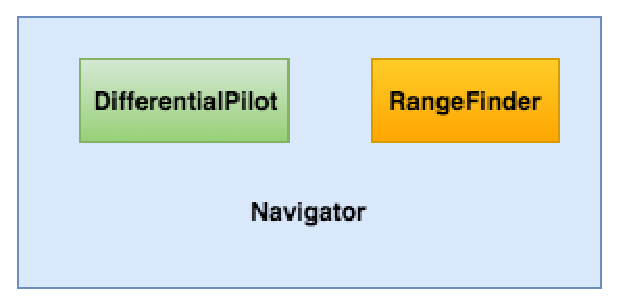
\includegraphics[scale=0.8]{figuras/classes_nav.eps}
		\caption[Classes Piloto]{Classes que contemplam o Piloto da solução.}
		\label{img:classes_navegacao}
	\end{figure}

	\subsection{Módulo Remoto - PC}

		A parte da solução que é executada remotamente envolve o processamento do Filtro de Partículas bem como a geração e o envio de comandos ao robô, seja para navegação
		ou obtenção de informações dos sensores. A solução possui um mecanismo de conexão \textit{bluetooth} com dispositivos, utilizando a ferramenta
		\textit{Bluecove}, bastando apenas informar o nome do dispositivo, que, no caso desta pesquisa, é \textbf{GTX}.

		A forma de \textit{input} desta informação é a partir da utilização do componente gráfico presente na API leJOS, o qual possibilita a apresentação do ambiente de navegação,
		as partículas e o resultado da filtragem, por exemplo, além da possibilidade do contato com o usuário por meio de \textit{inputs} textuais e botões.

		A Figura \ref{img:frame_pc} apresenta um exemplo do componente gráfico utilizado para contato com o usuário durante esta pesquisa.

		\begin{figure}[H]
			\centering
			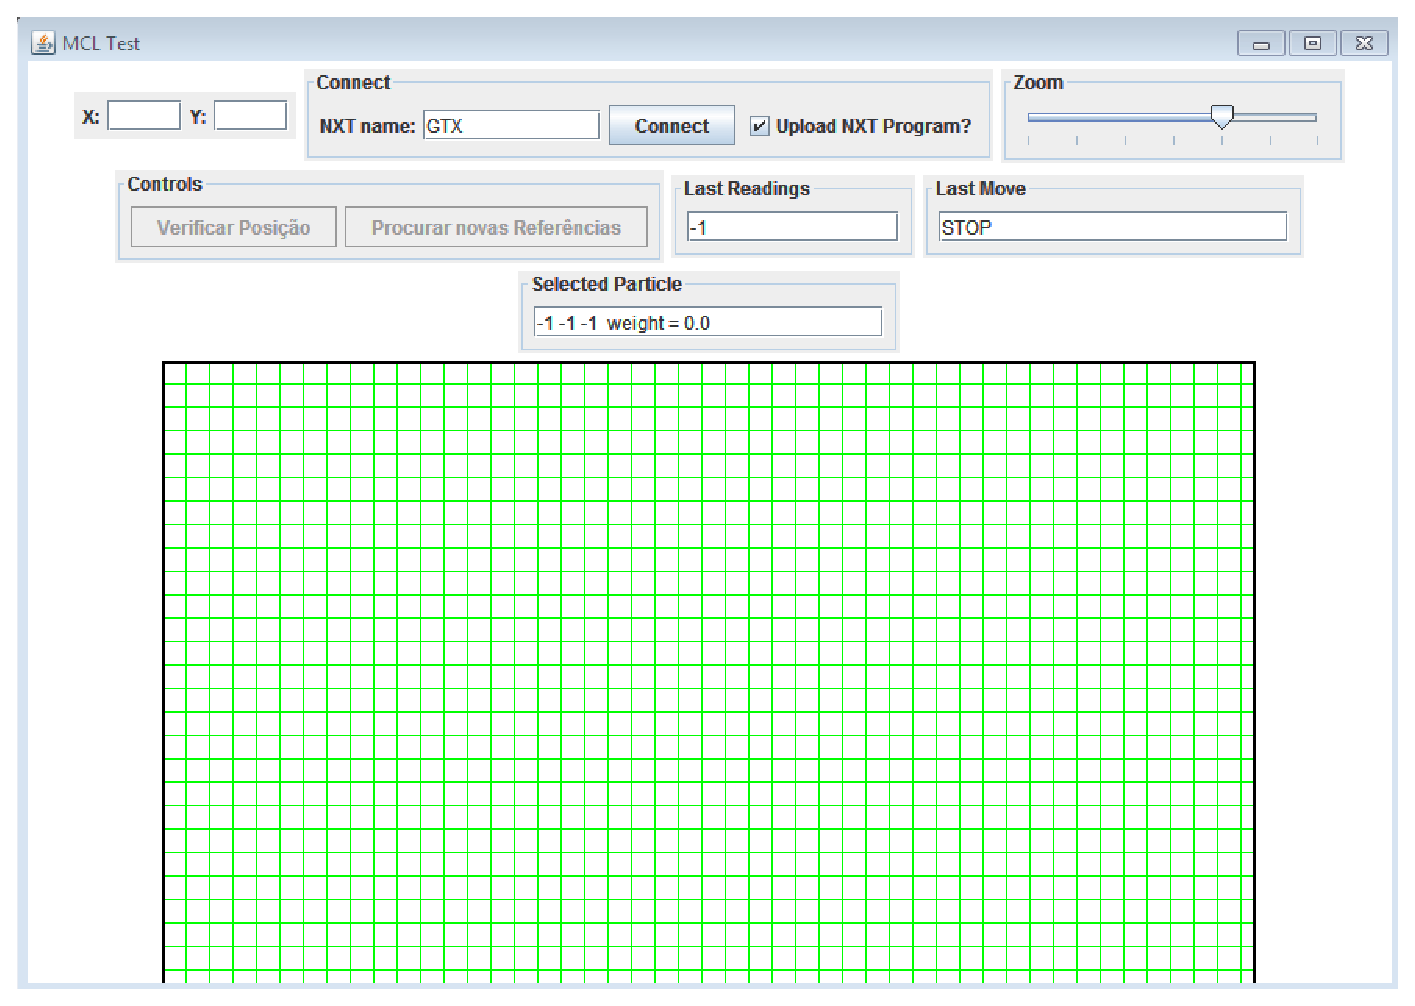
\includegraphics[scale=0.7]{figuras/frame.eps}
			\caption[Interface Gráfica]{Interface gráfica utilizada durante a pesquisa.}
			\label{img:frame_pc}
		\end{figure}

	A arquitetura de comunicação entre os projetos e o usuário segue o padrão apresentado na Figura \ref{img:arq_pc}. O módulo \textit{Localization}
	faz referência à parte da solução que é executada remotamente, em um computador. E o módulo \textit{Navigator} é executado localmente, no NXT.

	\begin{figure}[H]
		\centering
		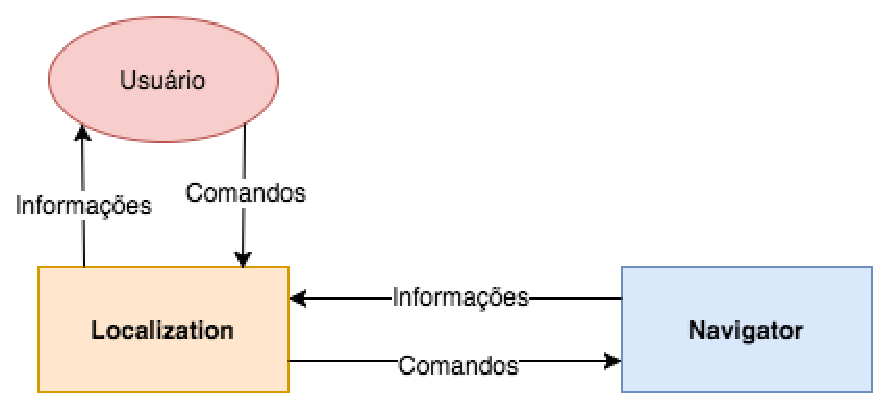
\includegraphics[scale=0.8]{figuras/arq_pc.eps}
		\caption[Arquitetura de Comunicação]{Arquitetura de Comunicação entre projetos e usuário.}
		\label{img:arq_pc}
	\end{figure}

O processamento do Filtro de Partículas é executado utilizando métodos da API leJOS, de acordo com toda a teoria apresentada na seção
\ref{sub:filtro_de_partículas}. A geração das informações de distância de cada partícula necessita de um processamento bastante elevado,
quando se tem como referência a capacidade de \textit{hardware} dos robôs NXT. Desse modo, todo esse processamento é feito remotamente,
executando em um computador. A quantidade de partículas utilizadas foi variável ao longo da pesquisa, buscando estudar o impacto desta variável
durante a execução dos testes. Dessa forma, conduziu-se um refinamento baseado em estudos empíricos.

\section{Considerações Parciais}

Durante este capítulo, foram apresentadas as caracteríticas técnicas da solução desenvolvida durante esta pesquisa, assim como o ambiente
utilizado para teste e o processo de configuração e instalação das ferramentas necessárias.

Esta solução foi desenvolvida e melhorada de forma que o principal objetivo foi analisar a viabilidade da utilização de uma técnica
de auto-localização utilizando o Kit de Robótica Mindstorms da Lego. Por esse motivo, foram utilizadas apenas ferramentas presentes no Kit
e em sua API, possibilitando a replicação do estudo e sua utilização em um ambiente Educacional por parte de qualquer interessado no assunto.
